
\subsection{Hardware Tests: Experiments and methods}

The functionality of the behaviours implemented can be tested individually.
Nevertheless, a more robust way of testing the behaviours is to combine them in certain test circuits that can be looped to check the reliability of these behaviours.
By building a more complex circuit to test, the different behaviours can be tested in different ways so the position of the robot changes before each of them.

This way, three different experiments have been executed to test the reliability of the robot:

\begin{enumerate}
	\item First, a test to check the robot is able to find, follow and get a good position on a line after right and left turning. 
With this test we can test the follow line, and turning behaviours.
The circuit used in this test was a "8", that means, the robot should turn left 4 times and then right 4 times in a row, 
as shown in figure \ref{fig:testMaps}.1.

	\item The second test executed has looked at the ability of the robot to go back in a intersection and turn to different directions after finding the previous intersection.
This test has been done running a circuit where the robot goes back, find the next intersection and goes back to the previous one. 
Then the robot turns in different directions each time, checking the response of all of them in different cases, as these directions are mixed.

	\item Finally, a experiment with a can has been executed to test the robot hability to push and place correctly the can.
In this experiment, the robot has to use all the different behaviours to move the can from one position to another and then to the original position again.

\end{enumerate}

The circuits used in each experiments are shown in the figure \ref{TestMaps}

Each of the three experiments have been executed starting with a full power battery and the circuit set for each one has been repeated 20 times in up to 10 trials without a battery change or charge.
The time needed to complete the 20 laps has been measured for each trial.
This allows us to determine too the fucionality and response of the robot in long runs.

About the light sensors, they have been tested to measure their response to different ambient light levels and the efectivity of shielding these sensors has been proved.
The information about this research is attached in \_reftolightsensors.


\begin{figure}[H]
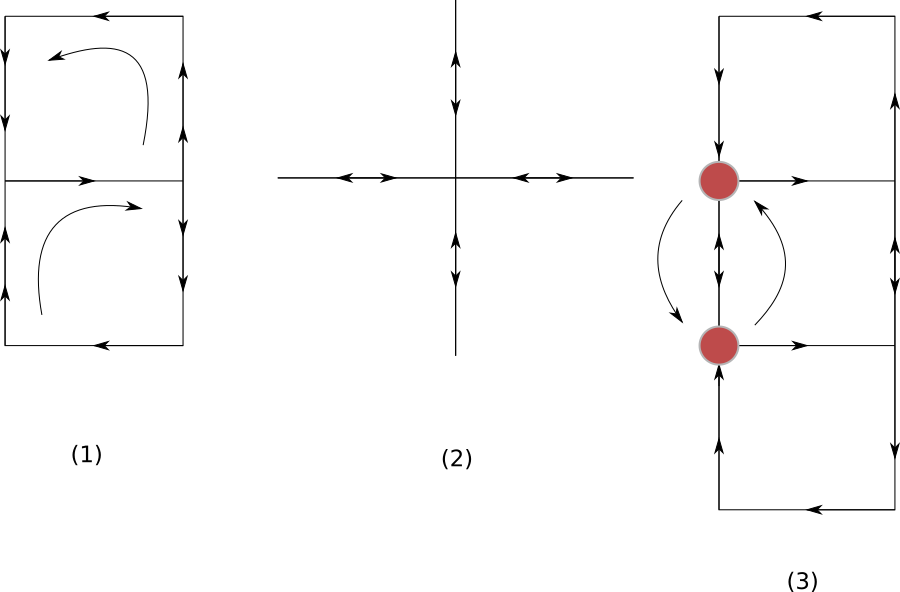
\includegraphics[width=10cm]{Test_circuits.png}
\centering
\caption{Scheme of the circuits used in the tests. 1, loop for turning behaviours. 2, used for pushing and going back behaviours. 3, used for testing the pushing behaviour with a can. }
\label{fig:testMaps}
\end{figure}



\begin{table}[H]
	\center
	
	\begin{tabular}{|l|c|r|c|r|c|r|}
	  	\cline{2-7}
	  	\multicolumn{1}{r}{}
 		&  \multicolumn{2}{|c|}{Experiment 1}
 		& \multicolumn{2}{|c|}{Experiment 2} 
 		& \multicolumn{2}{|c|}{Experiment 3}  
		 \\ \cline{2-7}
		\hline
		Run & Success & Time & Success & Time & Success & time \\
		\hline
		1 	& Yes & 6'26'' & Yes & 5'28'' & Yes & 8'16''\\
		2 	& Yes & 6'21'' & Yes & 5'33'' & Yes & 8'15''\\
		3 	& Yes & 6'27'' & Yes & 5'29'' & Yes & 8'17''\\
		4 	& Yes & 6'29'' & Yes & 5'30'' & Yes & 8'05''\\
		5 	& Yes & 6'33'' & Yes & 5'31'' & Yes & 8'15''\\
		6 	& Yes & 6'33'' & No  & 5'10'' & Yes & 8'10''\\
		7 	& Yes & 6'55'' & Yes & 5'34'' & Yes & 8'25''\\
		8 	& Yes & 6'52'' & Yes & 5'41'' & Yes & 8'54''\\
		9 	& No & LOWBAT  & No  & 1'13'' & No 	& LOWBAT\\
		10 	& No & LOWBAT  & No  & 1'50'' & No 	& LOWBAT\\		
		\hline
	\end{tabular}

	\caption{Table of results for the experiments. It is shown for each experiment and result the success or failure of the test and the time expended on it. In the case of the failed trials, the time shown represents the moment when the robot was lost. The LOWBAT statement means the robot finished his power and the experiment finished.}
	\label{tab:Experiment1}
\end{table}



